\documentclass[12pt,a4paper]{article}

% ================= PAQUETES =================
\usepackage[utf8]{inputenc}
\usepackage[T1]{fontenc}
\usepackage[spanish]{babel}
\usepackage{graphicx}
\graphicspath{{figs/}}
\usepackage{geometry}
\usepackage{fancyhdr}
\usepackage{listings}
\usepackage{xcolor}
\usepackage{float}
\usepackage{booktabs}
\usepackage{caption}
\usepackage{placeins} 
\usepackage{amsmath} 
\usepackage{tabularx}

% Estilo para el codigo del programa (.mem)
\lstdefinelanguage{memfile}{
  morecomment=[l]{//},
  sensitive=false
}
\lstdefinestyle{programa}{
  language=memfile,
  basicstyle=\ttfamily\footnotesize,
  commentstyle=\color{gray},
  numbers=left,
  numberstyle=\tiny\color{gray},
  numbersep=6pt,
  frame=single,
  xleftmargin=2em,
  framexleftmargin=1.5em,
  breaklines=true,
  columns=fixed,
  keepspaces=true,
  captionpos=b,
  aboveskip=1em,
  belowskip=1em,
  showstringspaces=false
}

% ================= MÁRGENES =================
\geometry{
  a4paper,
  margin=2.5cm,
  top=3.5cm,
  headheight=1.8cm,
  headsep=0.8cm
}

% ================= ENCABEZADO Y PIE =================

\pagestyle{fancy}
\fancyhf{}

\fancyhead[L]{
\includegraphics[height=1.6cm]{utec-logo}}
\fancyhead[R]{2026-2}

\fancyfoot[L]{Arquitectura de Computadoras (CS3051)}
\fancyfoot[R]{\thepage}
\renewcommand{\headrulewidth}{0.4pt}
\renewcommand{\footrulewidth}{0pt}

\begin{document}

% ================= PORTADA =================

\begin{center}
    \centering
    
\includegraphics[height=10cm]{utec-logo}\\
    \centering Arquitectura de Computadoras \\
    (CS3051) \\
    \vspace{1cm}
    {\large \textbf{Diseño e implementación de un procesador RISC-V superescalar Dual-Issue con optimización microarquitectónica}} \\
    \vspace{1cm}
    \centering
    {\Large \textbf{ \\ Proyecto 2 - Primera entrega }}
    \vspace{1cm}
    \begin{flushleft}
        \centering
        Alvarado León, Adriana Celeste            \\
        Daza Yalta, Gino Jesús                  \\
        Ccolcca Flores, Marylin Regina   \\  
        \vspace{3cm}
        \textbf{Profesor:} Williams Valencia , Carlos Eduardo\\ 
        
        \centering
        4 de noviembre del 2026
    \end{flushleft}
\end{center}

\newpage

% ================= ÍNDICE =================

\newpage
\thispagestyle{fancy} 
\vspace*{0.1cm}
\tableofcontents
\thispagestyle{fancy} 
\vspace*{0.1cm}
\newpage

% ================= CONTENIDO =================

\section{Introducción}

El presente proyecto tiene como objetivo diseñar e implementar un procesador RISC-V de 32 bits con arquitectura superescalar Dual-Issue, que sea capaz de emitir hasta dos instrucciones por ciclo. Como base, se desarrolla un procesador Pipeline Single-Issue de cinco etapas en Verilog, incorporando mecanismos de \textit{forwarding}, \textit{stalling} y \textit{flushing} para resolver dependencias de datos y riesgos de control.

En esta primera entrega, verificamos el funcionamiento del pipeline mediante programas de prueba e iniciamos su adaptación hacia una arquitectura Dual-Issue.

\subsection{Pipeline de Cinco Etapas}

El procesador implementa una arquitectura segmentada en cinco etapas, permitiendo que varias instrucciones se procesen simultáneamente en diferentes fases:

\begin{itemize}
    \item \textbf{Instruction Fetch (IF):} obtiene la instrucción desde memoria utilizando el Program Counter (PC). Normalmente, el PC avanza cuatro bytes, aunque puede actualizarse ante un salto o detenerse mediante \texttt{StallF}.

    \item \textbf{Instruction Decode (ID):} decodifica la instrucción, identifica los registros fuente y destino, lee los operandos del Register File y genera las señales de control.

    \item \textbf{Execute (EX):} ejecuta operaciones aritméticas y lógicas mediante la ALU, selecciona operandos y calcula las direcciones y condiciones de salto.

    \item \textbf{Memory Access (MEM):} realiza las operaciones de lectura y escritura sobre la memoria de datos, utilizando la dirección calculada en EX.

    \item \textbf{Write Back (WB):} selecciona y escribe en el Register File el resultado proveniente de la ALU, la memoria o PC+4.
\end{itemize}

Las etapas están conectadas mediante cuatro registros de pipeline: IF/ID, ID/EX, EX/MEM y MEM/WB. Estos conservan los datos y las señales de control correspondientes a cada instrucción. El procesador admite como máximo una nueva instrucción por ciclo, salvo cuando se requieren detenciones o anulaciones.

\subsection{Datapath}

El datapath, implementado en \texttt{datapath.v}, integra los registros de pipeline, el Register File, la ALU, los sumadores y los multiplexores necesarios para ejecutar las instrucciones.

En IF, el PC determina la dirección de lectura y se calcula PC+4. En ID, se identifican los registros fuente (\texttt{Rs1D}, \texttt{Rs2D}) y destino (\texttt{RdD}), se leen los operandos y se extiende el inmediato. El Register File dispone de dos puertos de lectura combinacional y uno de escritura en el flanco de bajada del reloj.

En EX, los multiplexores controlados por \texttt{ForwardAE} y \texttt{ForwardBE} seleccionan los operandos del Register File o los resultados adelantados desde MEM y WB. La señal \texttt{ALUSrcE} permite seleccionar un inmediato como segundo operando de la ALU.

Posteriormente, el resultado se transfiere a MEM para realizar los accesos correspondientes. En WB, \texttt{ResultSrcW} selecciona el dato que se escribirá en el registro destino. El datapath también incorpora la actualización del PC mediante \texttt{PCSrcE} y las conexiones necesarias para el control de hazards.

\subsection{Unidad de Control}

La unidad de control, implementada en \texttt{controller.v}, interpreta las instrucciones y genera las señales que coordinan el datapath. Está compuesta principalmente por los módulos \texttt{maindec.v} y \texttt{aludec.v}.

El módulo \texttt{maindec} decodifica el \textit{opcode} y genera señales como \texttt{RegWrite}, \texttt{MemWrite}, \texttt{ALUSrc}, \texttt{ResultSrc}, \texttt{ImmSrc}, \texttt{Branch} y \texttt{Jump}. Por su parte, \texttt{aludec} determina la operación de la ALU mediante \texttt{ALUOp}, \texttt{funct3} y \texttt{funct7}, generando \texttt{ALUControl}.

Las señales de control avanzan junto con cada instrucción mediante registros de pipeline, actuando en las etapas correspondientes. La resolución de saltos se realiza en EX mediante:

\begin{equation}
    PCSrcE = (BranchE \land ZeroE) \lor JumpE
\end{equation}

Asimismo, la unidad recibe \texttt{FlushE} desde la Hazard Unit para anular las señales de control de instrucciones que deben descartarse.

Esta organización modular permite coordinar la ejecución del procesador Single-Issue y constituye la base para su posterior extensión Dual-Issue.


\section{Hazard Unit y Datapath Single-Issue}

La arquitectura Pipeline Single-Issue incorpora una Hazard Unit, implementada en \texttt{hazard.v}, para gestionar dependencias de datos y riesgos de control. Esta unidad se conecta con el datapath y el controlador mediante \texttt{riscv.v}, implementando tres mecanismos principales: \textit{forwarding}, \textit{stalling} y \textit{flushing}.

\subsection{Cambios e Implementación de la Hazard Unit}

La incorporación de la Hazard Unit requirió añadir multiplexores de forwarding y registros de pipeline con señales de habilitación y limpieza. Su lógica combinacional compara registros fuente y destino de distintas etapas y genera las señales \texttt{ForwardAE}, \texttt{ForwardBE}, \texttt{StallF}, \texttt{StallD}, \texttt{FlushD} y \texttt{FlushE}.

\paragraph{a) Forwarding}

El forwarding permite resolver dependencias RAW (\textit{Read After Write}) utilizando resultados de instrucciones anteriores sin esperar su escritura en el Register File.

La unidad compara los registros fuente en Execute (\texttt{Rs1E}, \texttt{Rs2E}) con los destinos en Memory y Write Back (\texttt{RdM}, \texttt{RdW}). Las señales \texttt{ForwardAE} y \texttt{ForwardBE} controlan los multiplexores de operandos según la siguiente codificación:

\begin{center}
\begin{tabular}{|c|l|}
\hline
\textbf{Selección} & \textbf{Origen del operando} \\
\hline
00 & Register File \\
01 & Write Back (\texttt{ResultW}) \\
10 & Memory (\texttt{ALUResultM}) \\
\hline
\end{tabular}
\end{center}

La lógica prioriza los resultados de MEM sobre WB, seleccionando el valor más reciente cuando existen coincidencias. Además, se evita realizar forwarding desde escrituras cuyo destino es \texttt{x0}.

\paragraph{b) Stalling}

El stalling se utiliza cuando una instrucción depende de un dato que todavía no está disponible, como ocurre en una dependencia Load-Use.

La condición implementada en \texttt{hazard.v} es:

\begin{equation}
\begin{split}
\texttt{lwStallD} = \texttt{ResultSrcEb0} \land {}\\
((\texttt{Rs1D}=\texttt{RdE}) \lor
(\texttt{Rs2D}=\texttt{RdE}))
\end{split}
\end{equation}

Cuando se detecta esta dependencia, se activan \texttt{StallF} y \texttt{StallD}, deteniendo el PC y conservando la instrucción en IF/ID. Simultáneamente, \texttt{FlushE} limpia ID/EX e introduce una burbuja.

Para ello, el datapath utiliza los módulos \texttt{flopenr}, \texttt{flopenrc} y \texttt{floprc}, que permiten habilitar o limpiar los registros correspondientes.

\paragraph{c) Flushing}

El flushing descarta instrucciones del camino incorrecto cuando se produce un salto tomado. En la implementación, los saltos se resuelven en Execute mediante:

\begin{equation}
\texttt{PCSrcE} =
(\texttt{BranchE} \land \texttt{ZeroE})
\lor \texttt{JumpE}
\end{equation}

Cuando \texttt{PCSrcE} se activa, la Hazard Unit genera \texttt{FlushD} y \texttt{FlushE}, anulando las instrucciones más jóvenes ubicadas en IF e ID. Asimismo, el PC se actualiza con la dirección objetivo del salto.

La señal \texttt{FlushE} también limpia las señales de control del registro ID/EX, evitando escrituras incorrectas en registros o memoria.

\subsection{Diagrama del Datapath Single-Issue}

El datapath Single-Issue integra las cinco etapas del pipeline, los registros intermedios IF/ID, ID/EX, EX/MEM y MEM/WB, así como las rutas de forwarding y las conexiones con la Hazard Unit.

La Figura~\ref{fig:datapath-hazards} presenta el datapath de referencia con los multiplexores de selección de operandos y las señales que permiten detener o limpiar los registros del pipeline.

\begin{figure}[!htbp]
    \centering
    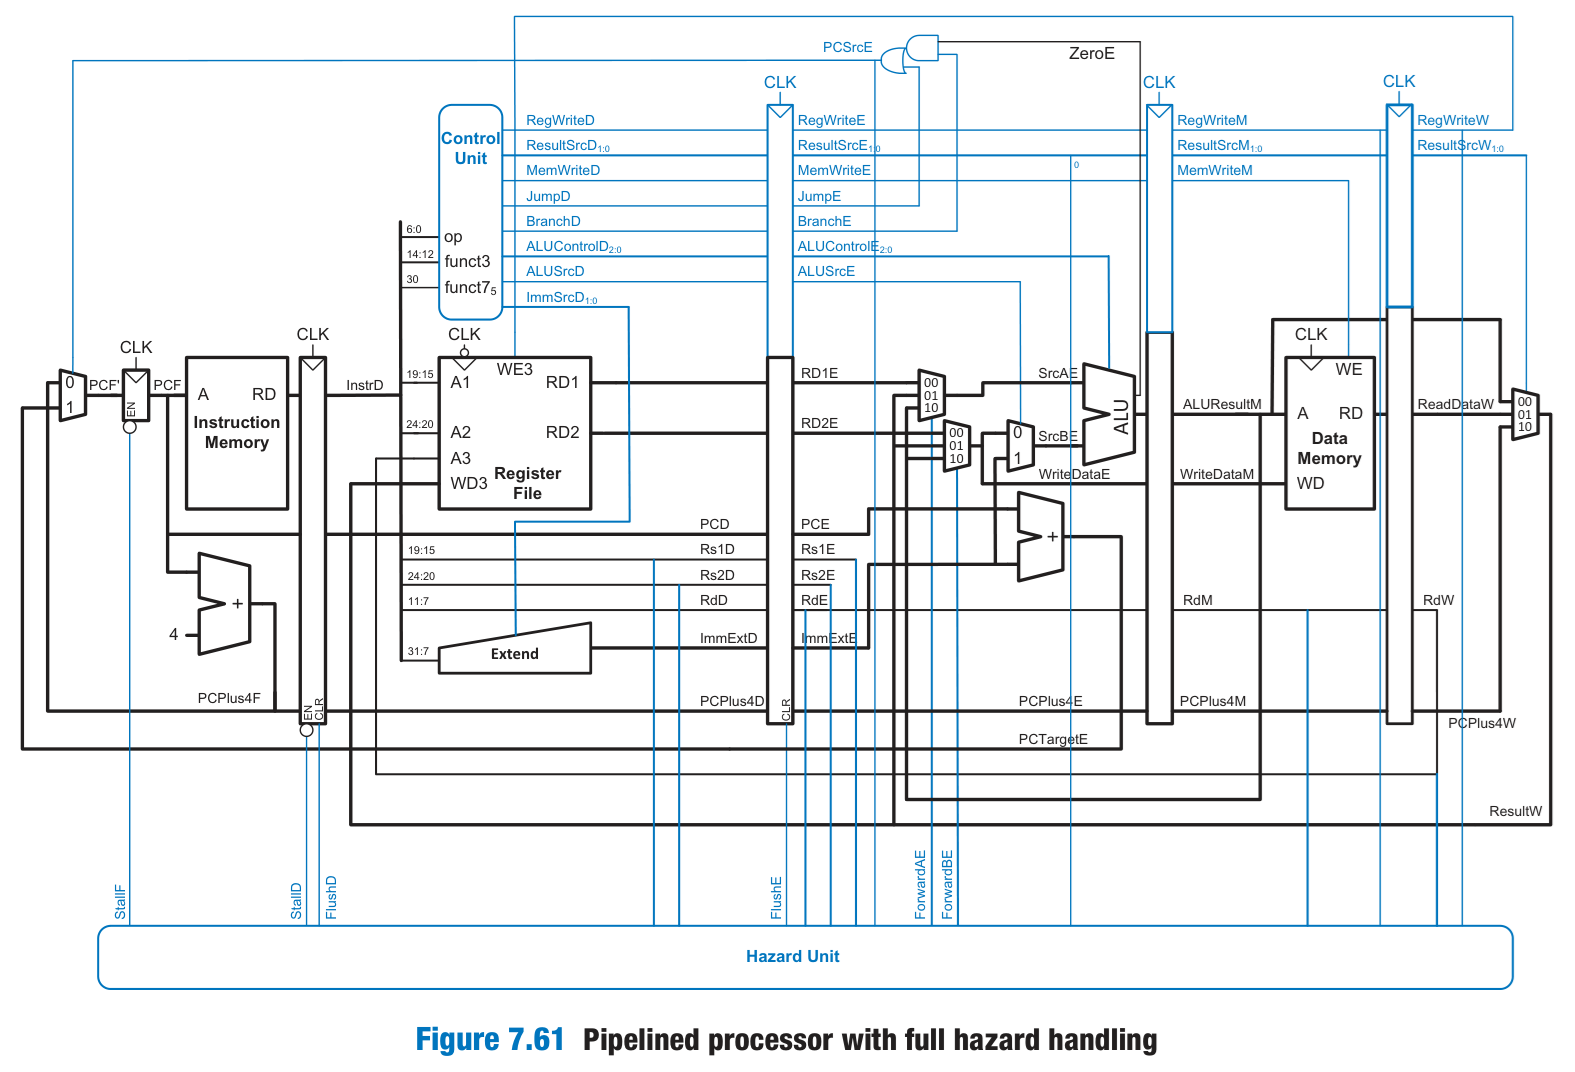
\includegraphics[
        width=\linewidth,
        height=0.36\textheight,
        keepaspectratio,
        trim=0 61.5bp 0 0,
        clip
    ]{pipeline-processor}
    \caption{Datapath pipeline Single-Issue con mecanismos de resolución de hazards.}
    \label{fig:datapath-hazards}
\end{figure}

La Figura~\ref{fig:singleissue-top} muestra la integración de los módulos de la implementación. En \texttt{riscv.v} se conectan el datapath, el controlador y la Hazard Unit, mientras que \texttt{top.v} incorpora las memorias de instrucciones y datos.

\begin{figure}[!htbp]
    \centering
    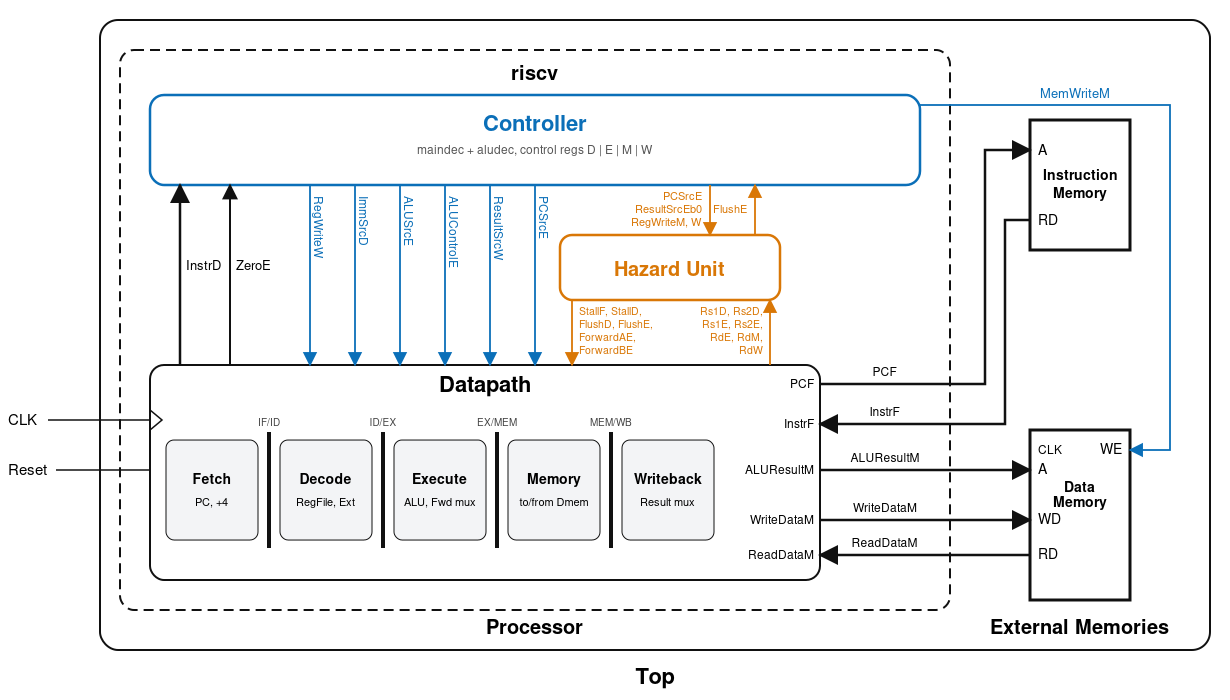
\includegraphics[
        width=0.92\linewidth,
        height=0.32\textheight,
        keepaspectratio
    ]{pipeline-top}
    \caption{Integración de los módulos del procesador Pipeline Single-Issue.}
    \label{fig:singleissue-top}
\end{figure}

\FloatBarrier

\section{Waveforms de los Cuatro Programas}

% ---------- PROGRAMA 1 ----------
\subsection{Programa 1} 

El Programa 1 verifica el funcionamiento básico del pipeline de cinco etapas ejecutando las instrucciones soportadas por el procesador en una secuencia donde ninguna instrucción depende de otra a menos de tres posiciones. Con esta separación, el valor producido ya fue escrito en el banco de registros cuando se necesita (este escribe en el flanco de bajada del reloj), por lo que no se requiere forwarding, stalling ni flushing. \\

\captionsetup[lstlisting]{labelformat=empty}
\begin{lstlisting}[style=programa, caption={Programa 1: ISA sin dependencias (\texttt{pipeline/isa.mem}).}, label={lst:p1}]
// Program 1 - ISA without dependencies that need the Hazard Unit
// Every consumer is 3+ instructions after its producer, so no forwarding/stall/flush.
// Expected stores: MEM[0]=17 [4]=7 [8]=8 [12]=17 [16]=1
00C00093  //   0: addi x1, x0, 12       ; x1 = 12
00500113  //   4: addi x2, x0, 5        ; x2 = 5
00A06193  //   8: ori x3, x0, 10        ; x3 = 10
00102393  //  12: slti x7, x0, 1        ; x7 = 1
00208233  //  16: add x4, x1, x2        ; 17
402082B3  //  20: sub x5, x1, x2        ; 7
0030F333  //  24: and x6, x1, x3        ; 8
00402023  //  28: sw x4, 0(x0)          ; MEM[0] = 17
00002483  //  32: lw x9, 0(x0)          ; x9 = 17
00502223  //  36: sw x5, 4(x0)          ; MEM[4] = 7
00602423  //  40: sw x6, 8(x0)          ; MEM[8] = 8
00902623  //  44: sw x9, 12(x0)         ; MEM[12] = 17 (from the lw)
00702823  //  48: sw x7, 16(x0)         ; MEM[16] = 1
0000006F  //  52: jal x0, 0             ; end: loop forever
\end{lstlisting}

\begin{figure}[H]
  \centering
  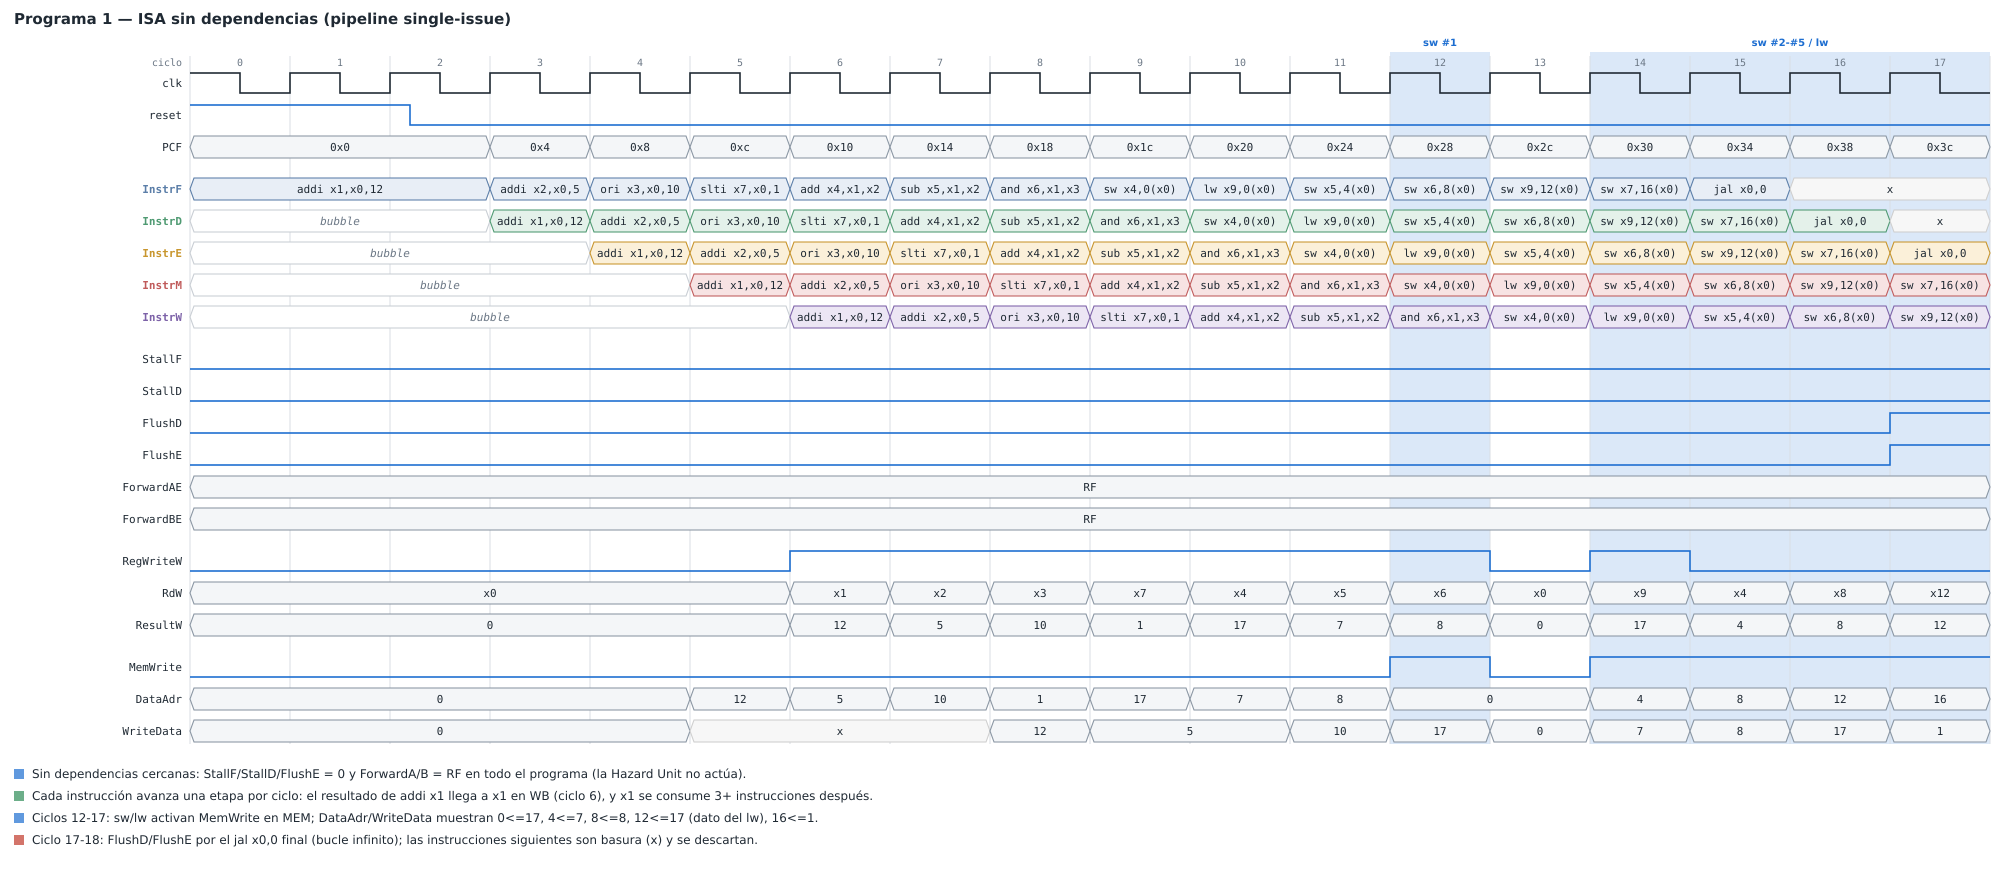
\includegraphics[width=\textwidth]{waveform-isa}
  \caption{Waveform de la ejecución del Programa 1.}
  \label{fig:wave_p1}
\end{figure}

\textbf{Análisis.} En la Figura~\ref{fig:wave_p1} se observa que la Hazard Unit no interviene mientras se ejecutan las instrucciones del programa: \texttt{ForwardAE} y \texttt{ForwardBE} se quedan en RF (\texttt{00}), y \texttt{StallF} y \texttt{StallD} valen 0 en todo momento. \texttt{FlushD} y \texttt{FlushE} solo se activan en el ciclo 17, por el \texttt{jal} final. Esto pasa porque ninguna instrucción usa un registro que se calculó hace menos de tres instrucciones. Por ejemplo, \texttt{add x4,x1,x2} (dirección 16) necesita x1 y x2, que se calcularon en las direcciones 0 y 4. El valor de x1 ya está escrito cuando \texttt{add} llega a Decode (ciclo 7), y el de x2 se escribe en ese mismo ciclo, como se explica a continuación.

El caso más justo ocurre cuando el valor se calculó tres instrucciones antes. Ahí el dato llega a tiempo porque el Register File escribe en el flanco de bajada del reloj: la instrucción que lo produce está en WB mientras la que lo necesita está en Decode, y esta alcanza a leer el valor nuevo en la misma mitad de ciclo, sin necesitar forwarding. Se ve con \texttt{sw x4,0(x0)} (dirección 28), que usa el x4 calculado por \texttt{add x4} (dirección 16): en el ciclo 10, \texttt{add} está en WB (\texttt{RdW}=x4, \texttt{ResultW}=17) y \texttt{sw} está en Decode.

Las escrituras en memoria se ven cuando cada \texttt{sw} llega a la etapa MEM y \texttt{MemWrite} se pone en 1 (ciclos 12 y 14 a 17; en el ciclo 13 está el \texttt{lw} y baja a 0). El \texttt{lw x9,0(x0)} lee el 17 que se guardó en \texttt{MEM[0]}, y luego \texttt{sw x9,12(x0)} lo copia a \texttt{MEM[12]}, lo que confirma que la lectura de memoria y la escritura en WB funcionan bien. Al final, el \texttt{jal x0,0} deja el programa en un bucle infinito; en el ciclo 17, cuando se resuelve en EX, se activan \texttt{FlushD} y \texttt{FlushE} y las instrucciones que venían después se descartan.


Los resultados de memoria coinciden con los esperados: en la waveform, cada vez que \texttt{MemWrite} vale 1, \texttt{DataAdr} y \texttt{WriteData} muestran $\texttt{MEM[0]}=17$, $\texttt{MEM[4]}=7$, $\texttt{MEM[8]}=8$, $\texttt{MEM[12]}=17$ y $\texttt{MEM[16]}=1$, que son los valores calculados a mano a partir del programa. Por lo tanto, el Programa 1 se ejecuta correctamente.



% ---------- FIN PROGRAMA 1 ----------

\subsection{Programa 2}


El Programa 2 verifica el \textit{forwarding} entre etapas. A diferencia
del Programa 1, aquí las instrucciones dependen de las inmediatamente
anteriores (dependencias de distancia 1 y 2), por lo que el valor
necesario aún no fue escrito en el banco de registros. La Hazard Unit
debe reenviarlo directamente desde la etapa de Memory o de Writeback hacia
la entrada de la ALU, sin detener el pipeline.

\begin{lstlisting}[style=programa, caption={Programa 2: Forwarding (\texttt{pipeline/forwarding.mem}).}, label={lst:p2}]
// Program 2 - Forwarding: back-to-back dependencies, no stalls
// Expected stores: MEM[0]=5 [4]=13 [8]=8
00500093  //   0: addi x1, x0, 5   ; x1 = 5
00308113  //   4: addi x2, x1, 3   ; x1 from MEM -> 8
001101B3  //   8: add  x3, x2, x1  ; x2 from MEM, x1 from WB -> 13
40218233  //  12: sub  x4, x3, x2  ; x3 from MEM, x2 from WB -> 5
00402023  //  16: sw   x4, 0(x0)   ; store data forwarded from MEM
00302223  //  20: sw   x3, 4(x0)
00202423  //  24: sw   x2, 8(x0)
0000006F  //  28: jal  x0, 0
\end{lstlisting}

\begin{figure}[H]
  \centering
  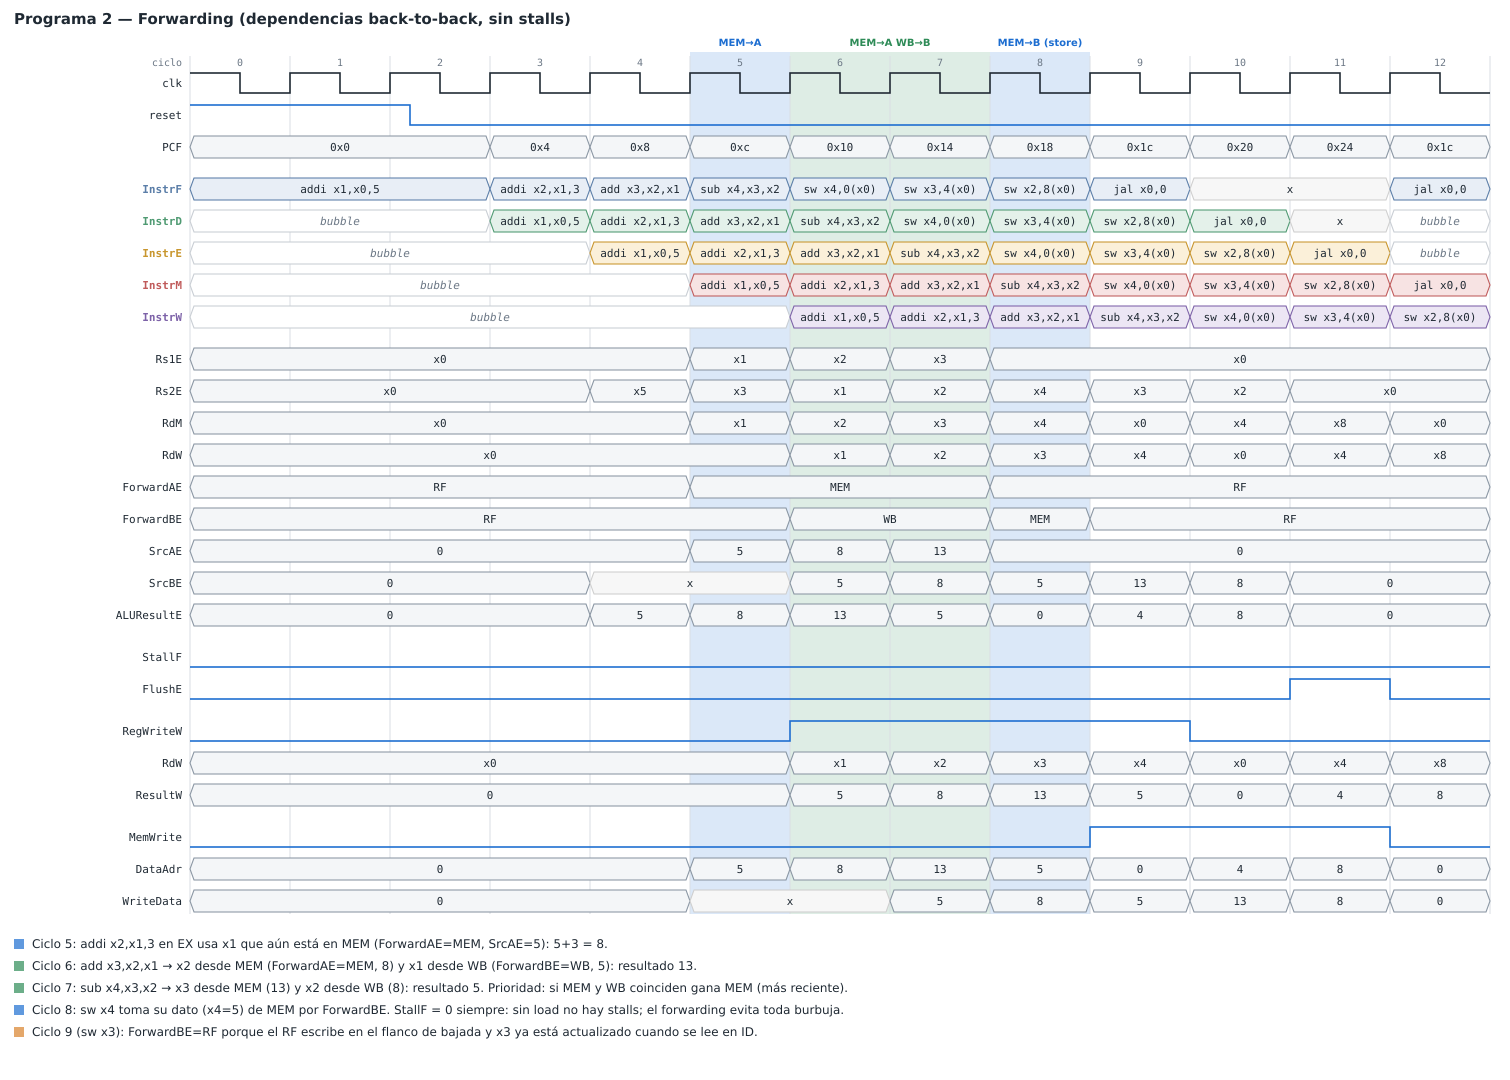
\includegraphics[width=\textwidth]{waveform-forwarding}
  \caption{Waveform de la ejecución del Programa 2.}
  \label{fig:wave_p2}
\end{figure}

\textbf{Análisis.} En la Figura~\ref{fig:wave_p2} cada instrucción necesita el resultado de la anterior. Ese resultado se calcula en la etapa EX, pero recién se escribe en el Register File (RF) cuando la instrucción llega a WB, dos etapas después. Mientras tanto, la instrucción siguiente ya está en Execute y necesita el valor. El \textit{forwarding} resuelve esto enviando el resultado directamente desde la etapa MEM o WB a la entrada de la ALU, sin esperar a que se escriba en el RF y sin detener el pipeline.

En el ciclo 5, \texttt{addi x2,x1,3} toma x1 desde MEM (\texttt{ForwardAE}=MEM, \texttt{SrcAE}=5) y calcula $5+3=8$. En el ciclo 6, \texttt{add x3,x2,x1} toma x2 desde MEM (8) y x1 desde WB (5), y da 13. En el ciclo 7, \texttt{sub x4,x3,x2} toma x3 desde MEM (13) y x2 desde WB (8), y da 5. En el ciclo 8, \texttt{sw x4} recibe x4=5 desde MEM por \texttt{ForwardBE}. Los \texttt{sw x3} y \texttt{sw x2} de los ciclos 9 y 10 ya no necesitan forwarding (\texttt{ForwardBE}=RF), porque el RF escribe en el flanco de bajada y ya tiene esos valores.

Gracias al forwarding, \texttt{StallF} vale 0 en todo el programa y no hay burbujas. \texttt{FlushE} solo sube en el ciclo 11, por el \texttt{jal} final. Las escrituras en memoria (ciclos 9 a 11) son $\texttt{MEM[0]}=5$, $\texttt{MEM[4]}=13$ y $\texttt{MEM[8]}=8$, iguales a los valores esperados, por lo que el Programa 2 se ejecuta correctamente.

\subsection{Programa 3}

El Programa 3 verifica el \textit{stalling} ante un hazard de tipo
load-use. Cuando una instrucción necesita el resultado de un \texttt{lw}
que está inmediatamente antes, el dato recién está disponible al final de
la etapa Memory, por lo que el forwarding por sí solo no alcanza. La
Hazard Unit detiene Fetch y Decode durante un ciclo e inserta una burbuja
en Execute; después, el dato se reenvía desde Writeback.

\begin{lstlisting}[style=programa, caption={Programa 3: Stalling (\texttt{pipeline/stall.mem}).}, label={lst:p3}]
// Program 3 - Stalling: load-use hazard (1 bubble)
// Expected stores: MEM[0]=42 [4]=43 [8]=86
02A00093  //   0: addi x1, x0, 42   ; x1 = 42
00102023  //   4: sw   x1, 0(x0)    ; MEM[0] = 42
00002103  //   8: lw   x2, 0(x0)    ; x2 = 42
00110193  //  12: addi x3, x2, 1    ; LOAD-USE: stall 1 cycle -> 43
00302223  //  16: sw   x3, 4(x0)    ; MEM[4] = 43
00402203  //  20: lw   x4, 4(x0)    ; x4 = 43
004202B3  //  24: add  x5, x4, x4   ; LOAD-USE on both operands: stall -> 86
00502423  //  28: sw   x5, 8(x0)    ; MEM[8] = 86
0000006F  //  32: jal  x0, 0
\end{lstlisting}

\begin{figure}[H]
  \centering
  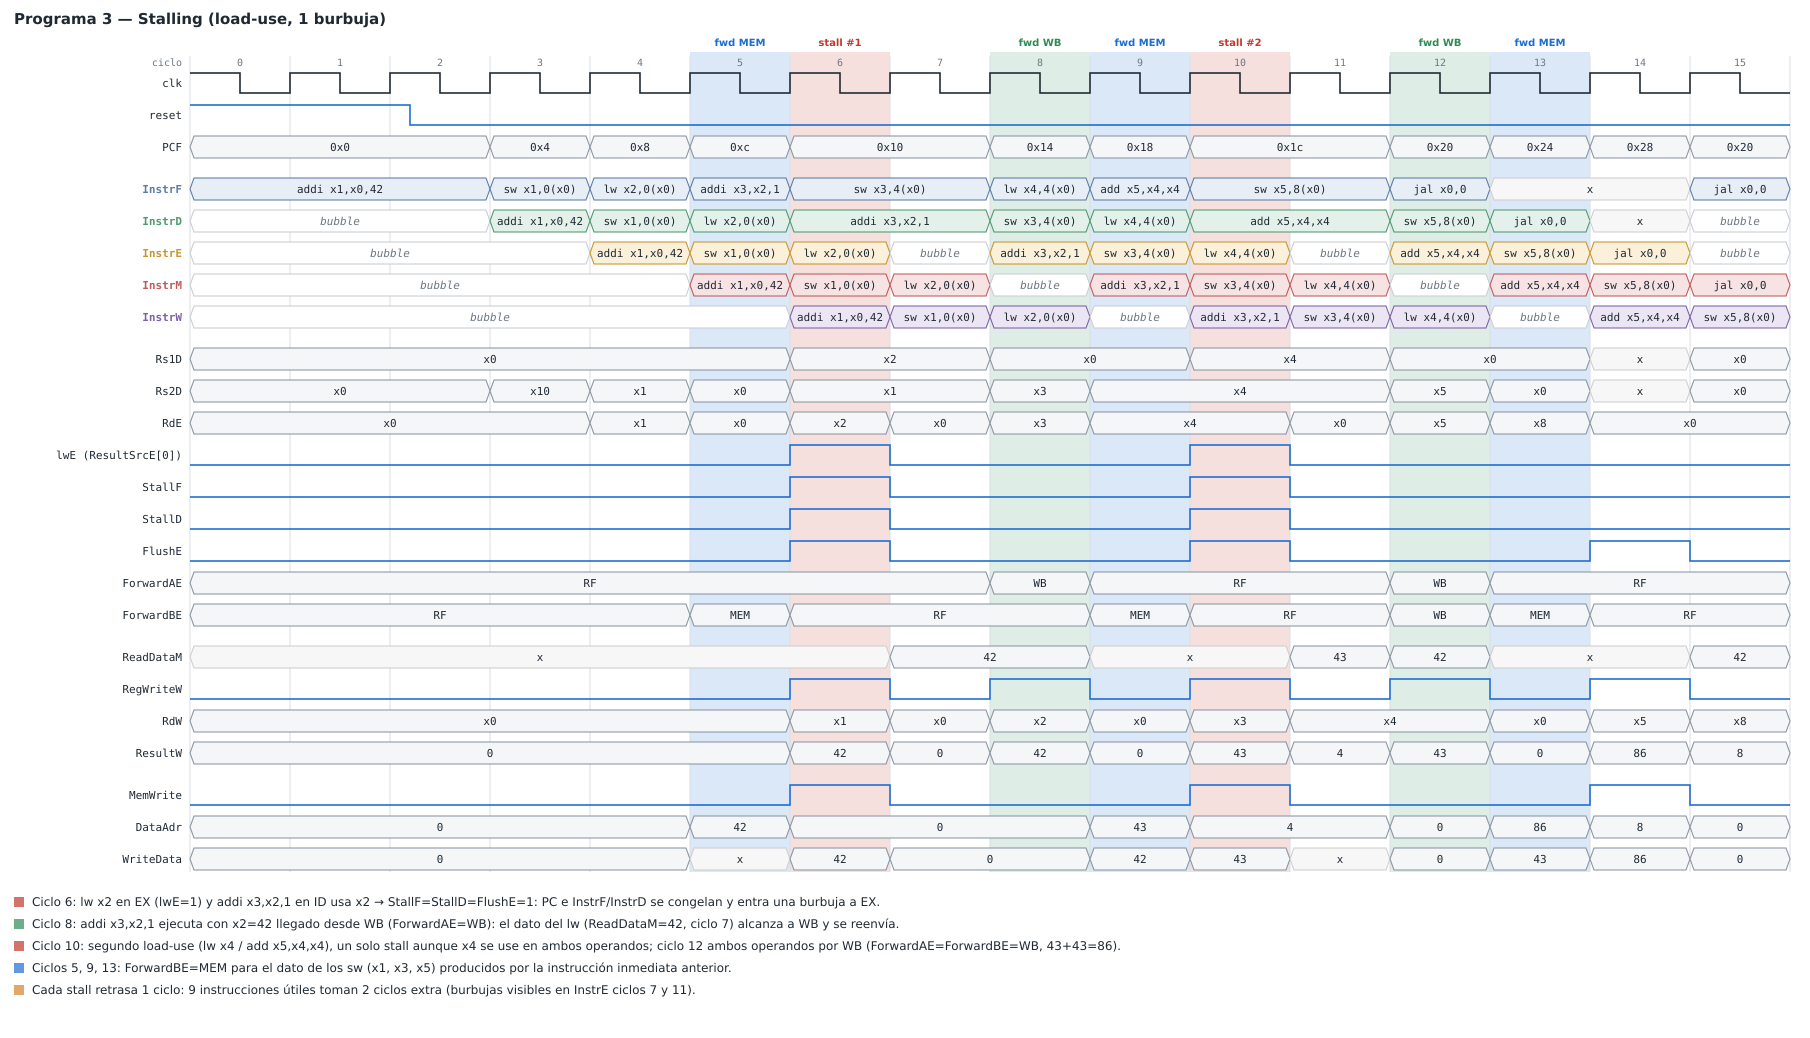
\includegraphics[width=\textwidth]{waveform-stall}
  \caption{Waveform de la ejecución del Programa 3.}
  \label{fig:wave_p3}
\end{figure}

\textbf{Análisis.} En la Figura~\ref{fig:wave_p3} hay dos casos de \textit{load-use}: una instrucción necesita el valor que carga un \texttt{lw} que está justo antes. El forwarding no alcanza aquí, porque el dato de un \texttt{lw} recién se lee de la memoria en la etapa MEM, y la instrucción siguiente ya está en Execute y lo necesita en ese mismo momento. La solución es un \textit{stall}: detener el pipeline un ciclo para que el dato llegue a tiempo. La Hazard Unit lo detecta cuando la instrucción en EX es un \texttt{lw} (\texttt{lwE}=1) y su registro destino (\texttt{RdE}) es igual a un registro fuente de la instrucción que está en Decode (\texttt{Rs1D} o \texttt{Rs2D}).

En el ciclo 6, \texttt{lw x2,0(x0)} está en EX y \texttt{addi x3,x2,1} está en Decode y usa x2 (\texttt{RdE}=\texttt{Rs1D}=x2). Entonces \texttt{StallF}, \texttt{StallD} y \texttt{FlushE} suben a 1: el PC (que se queda en \texttt{0x10}) y la instrucción en Decode se congelan, y se inserta una burbuja en EX (\texttt{InstrE} muestra \textit{bubble} en el ciclo 7). En ese ciclo el \texttt{lw} pasa a MEM y \texttt{ReadDataM}=42. En el ciclo 8, \texttt{addi x3,x2,1} ya puede ejecutarse: el \texttt{lw} está en WB y \texttt{ForwardAE}=WB le envía x2=42, con lo que calcula $42+1=43$.

El segundo caso es el de \texttt{lw x4,4(x0)} seguido de \texttt{add x5,x4,x4}, que usa x4 en los dos operandos. Aun así, se necesita un solo stall (ciclo 10), porque ambos operandos dependen del mismo \texttt{lw}. En el ciclo 12, \texttt{ForwardAE} y \texttt{ForwardBE} valen WB, y la ALU calcula $43+43=86$. Los \texttt{sw} que van justo después de la instrucción que produce su dato (ciclos 5, 9 y 13) no necesitan stall, solo forwarding desde MEM (\texttt{ForwardBE}=MEM), como en el Programa 2.

Cada stall le cuesta un ciclo al programa, así que los dos stalls suman dos ciclos extra. Las escrituras en memoria se ven en los ciclos 6, 10 y 14 (\texttt{MemWrite}=1), con \texttt{DataAdr}/\texttt{WriteData} igual a $\texttt{MEM[0]}=42$, $\texttt{MEM[4]}=43$ y $\texttt{MEM[8]}=86$. Coinciden con los valores esperados, por lo que el Programa 3 se ejecuta correctamente.


\subsection{Programa 4}

El Programa 4 prueba el \textit{flushing}. Tiene un \texttt{beq} que se cumple y un \texttt{jal}, y después de cada salto hay dos instrucciones \texttt{addi} (con el valor 99) que pertenecen al camino equivocado y no deben ejecutarse. Si la Hazard Unit las descarta bien, el valor 99 nunca se escribe y en memoria queda el valor correcto.
\begin{lstlisting}[style=programa, caption={Programa 4: Flushing (\texttt{pipeline/flush.mem}).}, label={lst:p4}]
// Program 4 - Flushing: taken beq and jal
// Wrong-path instructions would write 99; they must be flushed.
// Expected stores: MEM[0]=7 [4]=28
00700193  //   0: addi x3, x0, 7    ; x3 = 7 (must stay 7)
00500093  //   4: addi x1, x0, 5
00500113  //   8: addi x2, x0, 5
00208663  //  12: beq  x1, x2, 12   ; taken -> skips next 2
06300193  //  16: addi x3, x0, 99   ; flushed
06300193  //  20: addi x3, x0, 99   ; flushed
00C0036F  //  24: jal  x6, 12      ; x6 = 28, skips next 2
06300193  //  28: addi x3, x0, 99   ; flushed
06300193  //  32: addi x3, x0, 99   ; flushed
00302023  //  36: sw   x3, 0(x0)    ; still 7 -> wrong path flushed
00602223  //  40: sw   x6, 4(x0)    ; 28 (return address)
0000006F  //  44: jal  x0, 0
\end{lstlisting}

\begin{figure}[H]
  \centering
  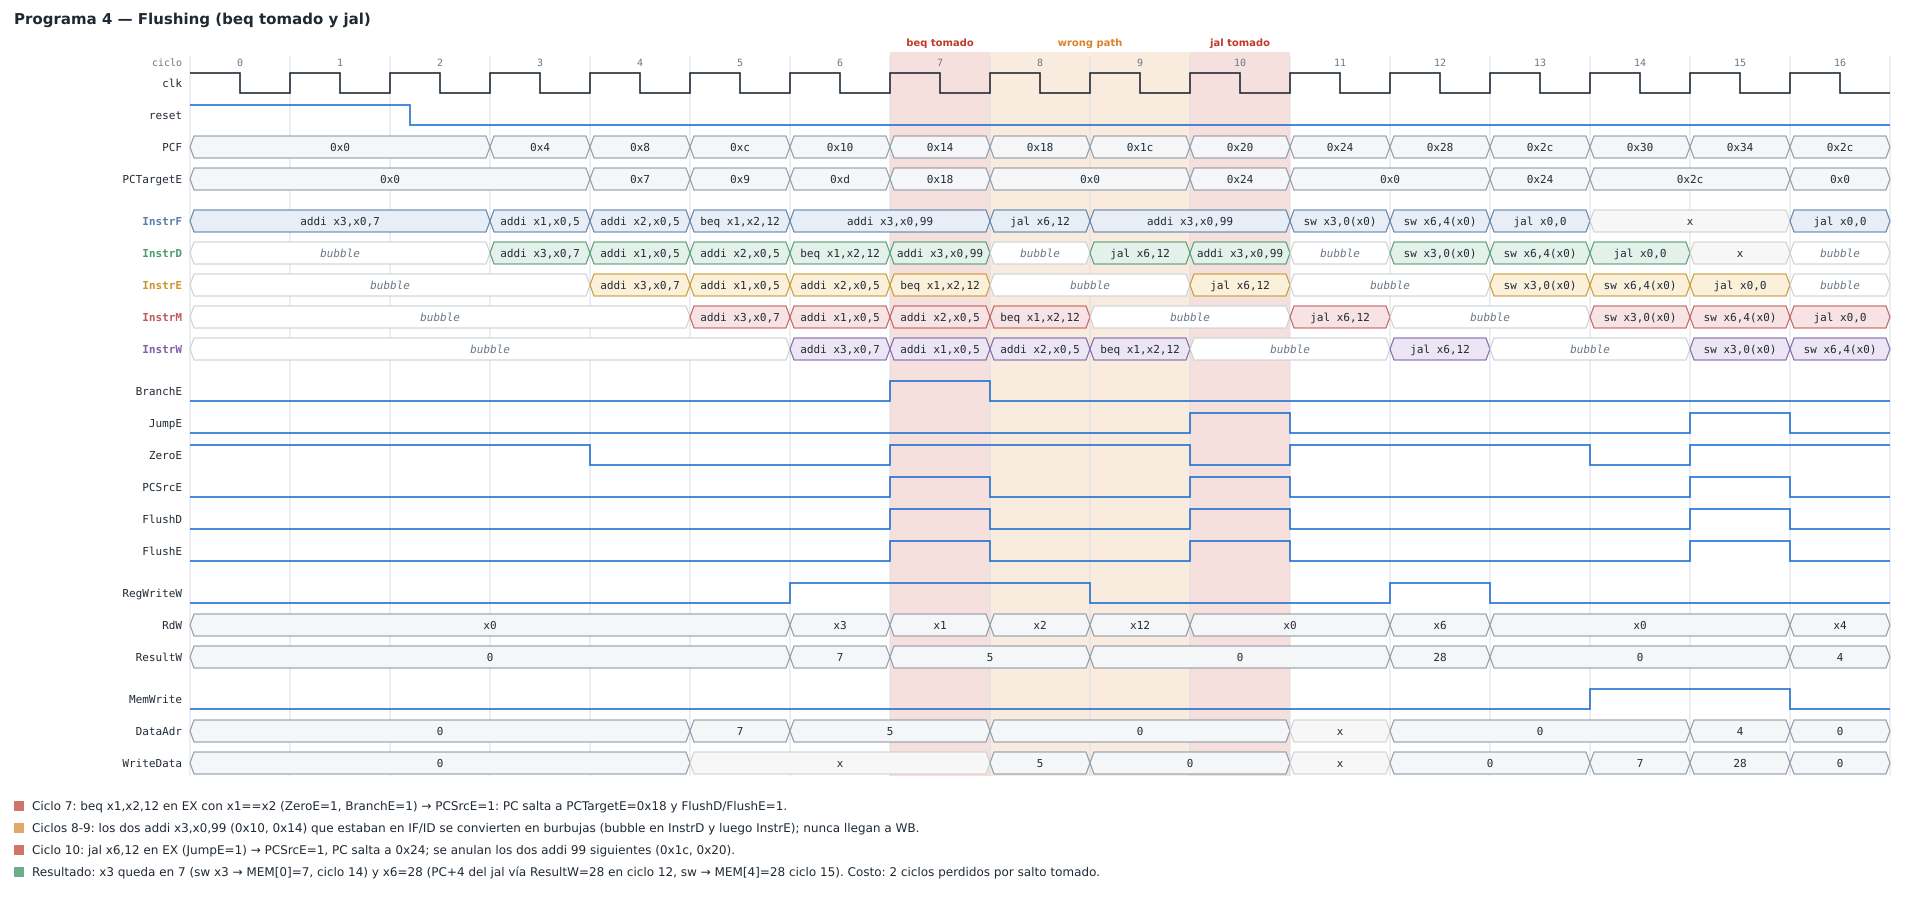
\includegraphics[width=\textwidth]{waveform-flush}
  \caption{Waveform de la ejecución del Programa 4.}
  \label{fig:wave_p4}
\end{figure}

\textbf{Análisis.} En la Figura~\ref{fig:wave_p4} se observa el \textit{flushing}. El procesador decide si un salto se toma recién en la etapa Execute, y para ese momento ya buscó las dos instrucciones que siguen al salto en el programa. Si el salto se toma, esas dos instrucciones son del camino equivocado y hay que descartarlas, porque si llegaran a ejecutarse modificarían registros o memoria. La Hazard Unit lo hace con \texttt{FlushD} y \texttt{FlushE}, que se activan cuando \texttt{PCSrcE}=1 y borran los registros IF/ID e ID/EX, convirtiendo esas instrucciones en burbujas.

En el ciclo 7, \texttt{beq x1,x2,12} está en EX. En ese mismo ciclo el \texttt{beq} recibe \texttt{x1} desde WB
(\texttt{ForwardAE}=WB) y \texttt{x2} desde MEM (\texttt{ForwardBE}=MEM), porque \texttt{x1} se calculó dos instrucciones antes y \texttt{x2} una antes,
y ninguno está todavía en el Register File. Como x1 y x2 valen 5, la ALU da cero (\texttt{ZeroE}=1), y con \texttt{BranchE}=1 se activa \texttt{PCSrcE}. El PC salta a \texttt{PCTargetE}=\texttt{0x18}, y \texttt{FlushD} y \texttt{FlushE} valen 1. Los dos \texttt{addi x3,x0,99} que ya estaban en el pipeline (direcciones \texttt{0x10} y \texttt{0x14}) se convierten en burbujas en los ciclos 8 y 9 (\textit{bubble} en \texttt{InstrD} e \texttt{InstrE}) y nunca llegan a WB. En el ciclo 10 ocurre lo mismo con \texttt{jal x6,12}: \texttt{JumpE}=1, \texttt{PCSrcE}=1, el PC salta a \texttt{0x24} y se descartan los dos \texttt{addi x3,x0,99} siguientes (\texttt{0x1c} y \texttt{0x20}).

El resultado confirma que el flush funcionó. Ninguna instrucción del camino equivocado llega a WB: en \texttt{ResultW} nunca aparece el 99. El primer \texttt{sw} escribe $\texttt{MEM[0]}=7$ en el ciclo 14, es decir, el valor correcto y no 99. Además, \texttt{jal x6,12} guarda la dirección de retorno PC+4 $=28$ (\texttt{RdW}=x6, \texttt{ResultW}=28 en el ciclo 12), y el segundo \texttt{sw} escribe $\texttt{MEM[4]}=28$ en el ciclo 15. Ambos valores coinciden con los esperados.


\subsection{Señales relevantes}

\begin{table}[H]
\centering
\begin{tabular}{lp{8.2cm}c}
\toprule
\textbf{Señal} & \textbf{Qué indica} & \textbf{Programa} \\
\midrule
\texttt{InstrF/D/E/M/W} & Instrucción que está en cada etapa del pipeline (solo para depurar) & 1--4 \\
\texttt{Rs1E}, \texttt{Rs2E}, \texttt{RdM}, \texttt{RdW} & Registros que compara la Hazard Unit para decidir el forwarding & 2 \\
\texttt{ForwardAE}, \texttt{ForwardBE} & Fuente de los operandos de la ALU: RF, WB o MEM & 1--4 \\
\texttt{SrcAE}, \texttt{SrcBE}, \texttt{ALUResultE} & Operandos que entran a la ALU y su resultado en Execute & 2 \\
\texttt{Rs1D}, \texttt{Rs2D}, \texttt{RdE}, \texttt{lwE} & Señales con las que se detecta el load-use: un \texttt{lw} en EX cuyo destino lo usa la instrucción en Decode & 3 \\
\texttt{StallF}, \texttt{StallD} & Congelan el PC y el registro IF/ID & 1--3 \\
\texttt{FlushD}, \texttt{FlushE} & Anulan las instrucciones en Decode y Execute (burbuja) & 1--4 \\
\texttt{BranchE}, \texttt{JumpE}, \texttt{ZeroE} & Salto condicional, salto incondicional y resultado cero de la ALU & 4 \\
\texttt{PCSrcE}, \texttt{PCTargetE} & Indica si se toma el salto y a qué dirección & 4 \\
\texttt{ReadDataM} & Dato que lee la memoria en la etapa MEM & 3 \\
\texttt{ResultW}, \texttt{RdW} & Valor y registro destino que se escriben en WB & 1--4 \\
\texttt{MemWrite}, \texttt{DataAdr}, \texttt{WriteData} & Escritura a memoria: cuándo, en qué dirección y con qué dato & 1--4 \\
\bottomrule
\end{tabular}
\caption{Señales relevantes observadas en las waveforms.}
\label{tab:senales}
\end{table}

\subsection{Resultados intermedios}

El Cuadro 2 resume lo observado en cada programa: el ciclo en que se hace el último \texttt{sw} y cuántas veces actuó la Hazard Unit (sin contar el \texttt{jal} final, que solo mantiene el bucle).

\begin{table}[H]
\centering
\begin{tabular}{lcccc}
\toprule
\textbf{Programa} & \textbf{Último \texttt{sw}} & \textbf{Forwardings} & \textbf{Stalls} & \textbf{Flushes} \\
\midrule
1 (ISA)         & ciclo 17 & 0 & 0 & 0 \\
2 (Forwarding)  & ciclo 11 & 6 & 0 & 0 \\
3 (Stalling)    & ciclo 14 & 6 & 2 & 0 \\
4 (Flushing)    & ciclo 15 & 2 & 0 & 2 \\
\bottomrule
\end{tabular}
\caption{Resumen de resultados por programa.}
\label{tab:resumen}
\end{table}

Algunos valores intermedios que se vieron en las waveforms: en el Programa 2, la ALU calculó 8, 13 y 5 (\texttt{ALUResultE}); en el Programa 3, el \texttt{lw} leyó 42 y 43 (\texttt{ReadDataM}) y la ALU calculó $42+1=43$ y $43+43=86$; en el Programa 4, \texttt{PCTargetE} valió \texttt{0x18} y \texttt{0x24}, y cada salto tomado descartó 2 instrucciones (2 ciclos perdidos).

\section{Implementación Preliminar del Dual-Issue}

La implementación preliminar Dual-Issue extiende el procesador Single-Issue mediante la obtención y decodificación paralela de dos instrucciones. En esta primera entrega, únicamente la vía 0 completa las etapas de ejecución, memoria y escritura. La segunda vía permanece preparada para su ampliación en la siguiente entrega.

\subsection{Cambios en Fetch}

Para leer dos instrucciones de 32 bits en el mismo ciclo, la etapa de \textit{Fetch} tuvo estas modificaciones:
\begin{itemize}
\item \textbf{Memoria de instrucciones de doble lectura (\texttt{imem}):} Se modificó para entregar al mismo tiempo la instrucción de la dirección $a$ y la siguiente, ubicada en $a+4$:
\begin{align}
rd1 &= RAM[a[31:2]] \\
rd2 &= RAM[a[31:2] + 1]
\end{align}
Así, en cada ciclo se obtienen \texttt{InstrF\_0} e \texttt{InstrF\_1}.

\item \textbf{Cálculo de PC+8:} Se agregó un sumador (\texttt{pcadd8}) que calcula $PC+8$, y el multiplexor del PC (\texttt{pcmux}) pasó a tener tres entradas: $PC+4$, $PC+8$ y la dirección del salto. En esta entrega el selector solo elige $PC+4$ o la dirección del salto, porque únicamente la vía 0 ejecuta instrucciones; por eso el PC avanza de 4 en 4. La entrada $PC+8$ queda lista para la segunda entrega, cuando la Issue Unit decida si emitir una o dos instrucciones por ciclo.

\item \textbf{Registro IF/ID más ancho:} El registro entre Fetch y Decode (\texttt{regD}, de tipo \texttt{flopenrc}) pasó de 96 a 192 bits para guardar las dos instrucciones, sus PC y sus PC+4: \texttt{InstrF\_0}, \texttt{InstrF\_1}, \texttt{PCF}, \texttt{PCPlus4F} y \texttt{PCPlus8F}. Mantiene las señales \texttt{StallD} y \texttt{FlushD}.
\end{itemize}

\subsection{Cambios en Decode}

La etapa de \textit{Decode} se modificó para decodificar las dos instrucciones del par en el mismo ciclo:
\begin{itemize}
\item \textbf{Decodificación paralela (\texttt{controller}):} Se instanciaron dos decodificadores idénticos (\texttt{maindec} y \texttt{aludec}), uno por cada vía. El de la vía 0 genera las señales de control de \texttt{InstrD\_0} (\texttt{RegWriteD\_0}, \texttt{ResultSrcD\_0}, \texttt{MemWriteD\_0}, \texttt{ALUSrcD\_0}, \texttt{ALUControlD\_0}, entre otras) y el de la vía 1 hace lo mismo con \texttt{InstrD\_1}. Cada vía tiene además sus propios registros de control entre etapas.
\item \textbf{Register File con 4 lecturas y 2 escrituras (\texttt{regfile}):} Para leer los operandos de ambas instrucciones a la vez, el Register File tiene cuatro puertos de lectura combinacionales y dos de escritura:
\begin{itemize}
\item Vía 0: \texttt{a1} $=$ \texttt{InstrD\_0[19:15]} y \texttt{a2} $=$ \texttt{InstrD\_0[24:20]} (salidas \texttt{rd1}, \texttt{rd2}).
\item Vía 1: \texttt{a4} $=$ \texttt{InstrD\_1[19:15]} y \texttt{a5} $=$ \texttt{InstrD\_1[24:20]} (salidas \texttt{rd4}, \texttt{rd5}).
\item Escritura: puertos \texttt{we3/a3/wd3} y \texttt{we6/a6/wd6}, ambos en el flanco de bajada del reloj. Si las dos vías escriben el mismo registro, gana la vía 1 (la instrucción más joven). En esta entrega solo se usa el puerto de la vía 0; el de la vía 1 queda deshabilitado (\texttt{RegWriteW\_1}$=0$) hasta completar su etapa de Writeback.
\end{itemize}
\item \textbf{Generadores de inmediato (\texttt{extend}):} Se instanciaron dos unidades de extensión de signo, \texttt{ext\_0} y \texttt{ext\_1}, que generan \texttt{ImmExtD\_0} e \texttt{ImmExtD\_1} en paralelo.
\end{itemize}

\subsection{Módulos incorporados}

Para pasar del pipeline Single-Issue a la versión Dual-Issue preliminar se modificaron los siguientes módulos:
\begin{itemize}
\item \texttt{imem.v}: memoria de instrucciones con dos salidas de 32 bits (\texttt{rd1} y \texttt{rd2}), que entregan la instrucción de la dirección $a$ y la siguiente.
\item \texttt{regfile.v}: Register File con 4 puertos de lectura y 2 de escritura.
\item \texttt{controller.v}: tiene dos copias de los decodificadores (\texttt{maindec} y \texttt{aludec}) y registros de control separados para cada vía.
\item \texttt{datapath.v}: incorpora el sumador \texttt{pcadd8}, el IF/ID de 192 bits, y la decodificación y el registro ID/EX de la vía 1. La ejecución, la memoria y el Writeback siguen solo en la vía 0.
\item \texttt{hazard.v}: se amplió con los puertos de la vía 1, pero por ahora la lógica de forwarding, stall y flush solo se calcula para la vía 0; las salidas de forwarding de la vía 1 están fijas en \texttt{00}. La detección de dependencias entre las dos vías queda para la segunda entrega.
\item \texttt{riscv.v} y \texttt{top.v}: conectan las señales de las dos vías entre el controller, el datapath, la Hazard Unit y la memoria de instrucciones (\texttt{InstrF\_0} e \texttt{InstrF\_1}).
\end{itemize}

El resto de los módulos (\texttt{alu}, \texttt{aludec}, \texttt{maindec}, \texttt{extend}, \texttt{dmem}, \texttt{mux2}, \texttt{mux3}, \texttt{adder} y los registros \texttt{flopr}, \texttt{floprc}, \texttt{flopenr} y \texttt{flopenrc}) se reutilizan sin cambios del pipeline Single-Issue.

\subsection{Datapath Dual-Issue Preliminar}

El datapath preliminar extiende el pipeline Single-Issue con una segunda vía (\textit{Lane 1}) que, por ahora, llega hasta la etapa de Decode: se leen y decodifican dos instrucciones por ciclo, pero solo la vía 0 (\textit{Lane 0}) ejecuta y escribe resultados. Esto permite verificar el Dual Fetch y el Dual Decode sin alterar el comportamiento ya validado con los cuatro programas.

\begin{itemize}
    \item \textbf{Fetch (IF):} \texttt{imem} entrega al mismo tiempo dos instrucciones consecutivas (\texttt{InstrF\_0} en la dirección \texttt{PCF} e \texttt{InstrF\_1} en \texttt{PCF}$+4$). El PC avanza de 4 en 4 (\texttt{PCPlus4F}); el sumador \texttt{pcadd8} y la entrada $PC+8$ del \texttt{pcmux} ya existen, pero se activarán en la segunda entrega.
    \item \textbf{Decode (ID):} el registro IF/ID (\texttt{regD}) tiene 192 bits y guarda las dos instrucciones, sus PC y sus PC+4. Cada instrucción tiene su propio decodificador de control, su generador de inmediato (\texttt{ext\_0}, \texttt{ext\_1}) y sus puertos de lectura del Register File (\texttt{rd1, rd2} y \texttt{rd4, rd5}). El registro ID/EX también está duplicado (\texttt{regE\_0} y \texttt{regE\_1}).
    \item \textbf{Execute (EX):} solo la vía 0 tiene ALU (\texttt{alu\_0}), multiplexores de forwarding (\texttt{faemux\_0} y \texttt{fbemux\_0}) y sumador de saltos (\texttt{pcaddbranch\_0}). La vía 1 no tiene todavía su ALU.
    \item \textbf{Memory y Writeback (MEM/WB):} la memoria de datos y la escritura en el Register File siguen asignadas a la vía 0 (\texttt{ALUResultM\_0} y \texttt{WriteDataM\_0}). El puerto de escritura de la vía 1 existe en el Register File (\texttt{we6}, \texttt{a6}, \texttt{wd6}), pero está deshabilitado (\texttt{RegWriteW\_1}$=0$).
\end{itemize}

\subsection{Evidencia del Dual Fetch y Dual Decode}

Para comprobar el Dual Fetch y el Dual Decode se ejecutó el Programa 1
(\texttt{pipeline/isa.mem}) sobre el pipeline Dual-Issue preliminar. La
Figura~\ref{fig:dual-p1} muestra la etapa Fetch, la decodificación de ambos
carriles (vías) y el avance de las instrucciones por el pipeline.

\begin{figure}[H]
  \centering
  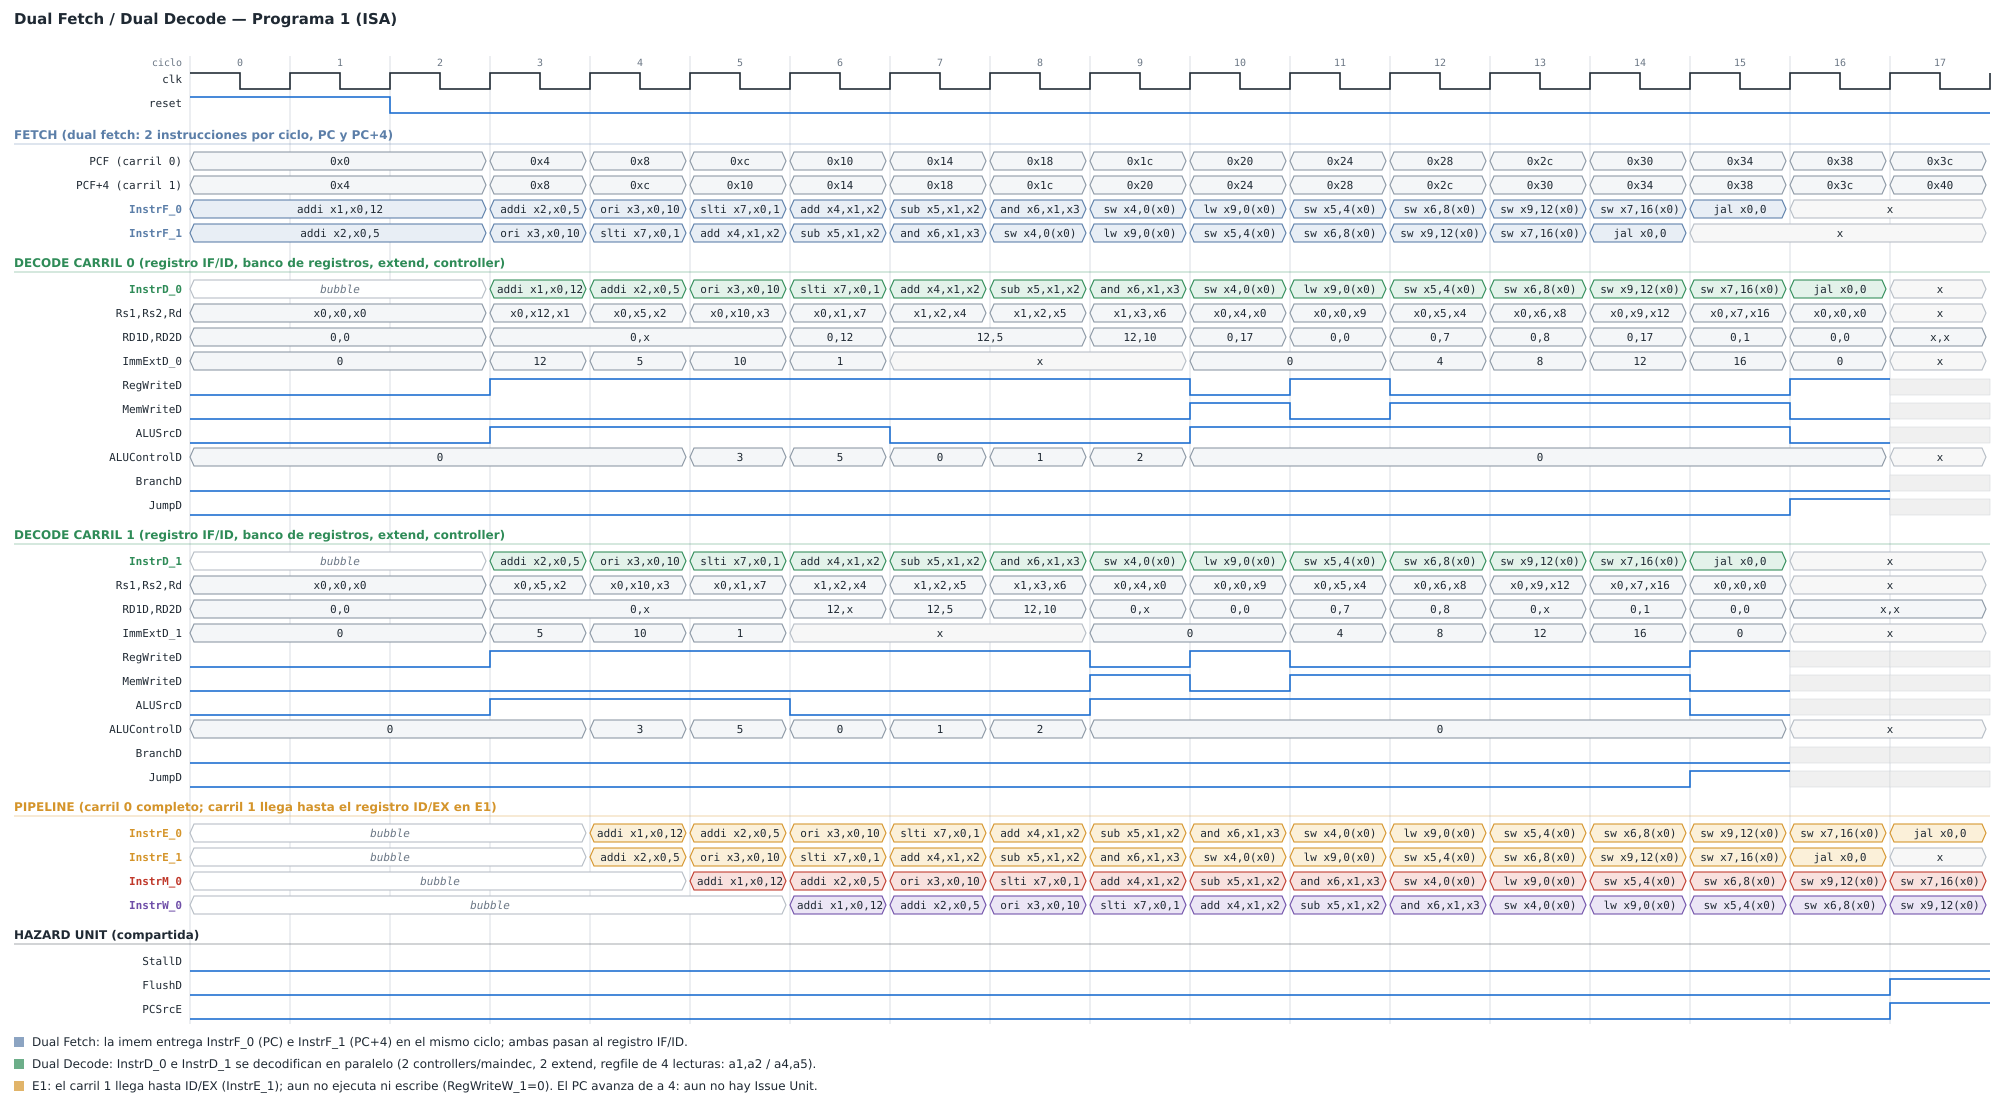
\includegraphics[width=\textwidth]{waveform-dual-fetch-decode}
  \caption{Waveform del Dual Fetch y Dual Decode (Programa 1).}
  \label{fig:dual-p1}
\end{figure}

\textbf{Dual Fetch.} En el ciclo 2, con \texttt{PCF}\,=\,\texttt{0x0}, la
memoria de instrucciones entrega al mismo tiempo \texttt{InstrF\_0}
(\texttt{addi x1,x0,12}) e \texttt{InstrF\_1} (\texttt{addi x2,x0,5}), que
corresponden a las direcciones \texttt{0x0} y \texttt{0x4}. En el ciclo 3 el
registro IF/ID ya contiene el par completo (\texttt{InstrD\_0} e
\texttt{InstrD\_1}), por lo que ambas instrucciones se capturan en el mismo
flanco. 

\textbf{Dual Decode.} En cada ciclo la etapa Decode toma las dos instrucciones
del registro IF/ID y las decodifica en paralelo: cada carril tiene su propio
decodificador de control (\texttt{maindec} y \texttt{aludec}), su generador de
inmediato y sus puertos de lectura del Register File (\texttt{rd1}, \texttt{rd2}
para el carril 0 y \texttt{rd4}, \texttt{rd5} para el carril 1). Esto se
evidencia en la Figura~\ref{fig:dual-p1}. En el ciclo 7, \texttt{add x4,x1,x2}
(carril 0) y \texttt{sub x5,x1,x2} (carril 1) leen los mismos registros por
puertos distintos (\texttt{RD1D},\texttt{RD2D}\,=\,12,\,5 en ambos carriles) y
solo difieren en \texttt{ALUControlD}: 0 para \texttt{add} y 1 para \texttt{sub}.
En el ciclo 9, el carril 0 decodifica \texttt{and x6,x1,x3} (tipo R,
\texttt{ALUControlD}\,=\,2) y el carril 1 decodifica \texttt{sw x4,0(x0)}
(tipo S): el carril 1 activa \texttt{MemWriteD} y \texttt{ALUSrcD}, apaga
\texttt{RegWriteD} y genera su inmediato (\texttt{ImmExtD\_1}\,=\,0), mientras
que el carril 0 mantiene \texttt{RegWriteD} activo y \texttt{MemWriteD} y
\texttt{ALUSrcD} en 0. Así, cada carril produce sus propias señales de control
según la instrucción que recibe, sin depender del otro.


\end{document}